\begin{figure}[!b]
\centering
\begin{subfigure}{0.8\textwidth}
    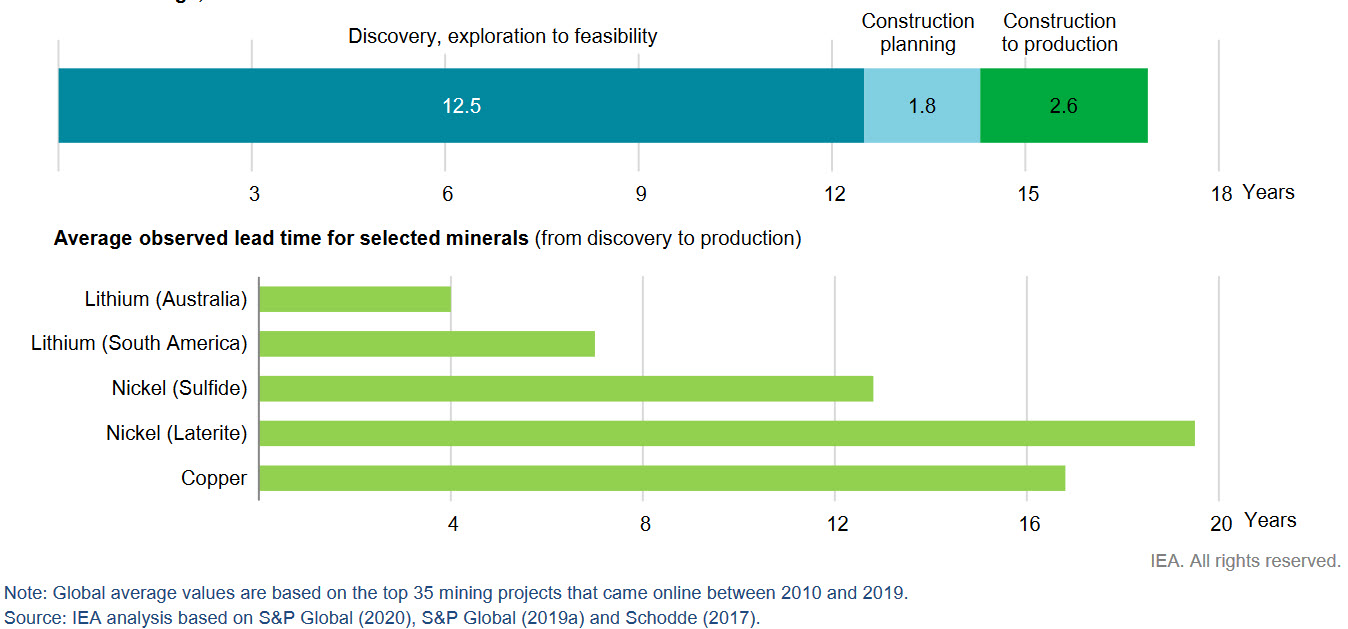
\includegraphics[width=\textwidth]{Images/supply_chain/Time_for_mining_2.jpg}
    \caption{Temps moyen de développement d'un site d'extraction minier (\cite{iea_role_2021})}
    \label{fig:Time_mining}
\end{subfigure}
\hfill
\begin{subfigure}{0.8\textwidth}
    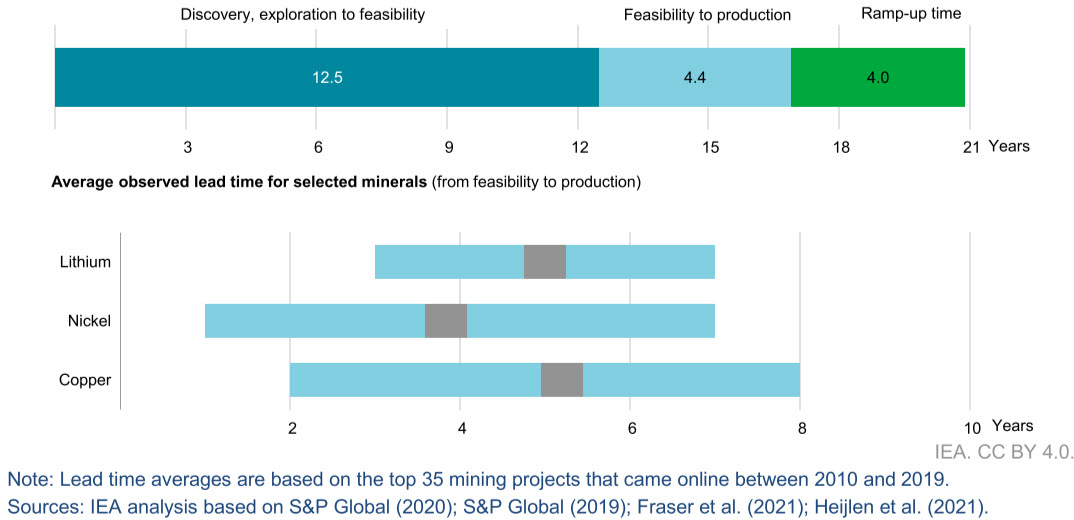
\includegraphics[width=\textwidth]{Images/supply_chain/Time_for_mining.jpg}
    \caption{Temps moyen de développement d'un site d'extraction minière (\cite{iea_energy_2023})}
    \label{fig:Time_mining_2}
\end{subfigure}

\caption{Temps moyen de développement d'un site minier}
\caption*{Note: En utilisant une méthode de calcul \textit{a priori} identique, l'AIE a réévalué à la hausse le temps moyen de développement d'un site minier.}
\label{fig:Time_mining_all}
\end{figure}

Le temps requis pour installer ou accroître une chaîne d'approvisionnement peut augmenter fortement le risque géopolitique. Les conséquences sur un pays d'un défaut d'approvisionnement en matériaux ou en équipements nécessaires à un système énergétique décarboné peut être plus ou moins important selon la durée requise pour rétablir des conditions d'approvisionnement satisfaisantes. Cette sous-section vise donc à donner les temporalités actuelles des différents maillons des chaînes d'approvisionnement. Plus l'augmentation de capacité d'un maillon est longue, plus les risques géopolitiques autour de ce maillon peuvent être amplifiés.\smallbreak
Le temps de développement de nouveaux sites miniers fait partie des plus élevés dans les chaînes d'approvisionnement des technologies bas-carbone (figure \ref{fig:Time_mining_all}). Le développement d'un site minier jusqu'à sa capacité nominale prend en moyenne près de 20 ans. L'exploration prend plus de 10 ans et n'aboutit pas nécessairement au développement d'un site minier. Le temps de construction du site est de l'ordre de 5 ans, mais il faut attendre à nouveau 5 ans pour que la mine atteigne sa capacité nominale de production. Au total, 15 ans en moyenne sont nécessaires pour qu'un site minier entre en production, puis encore plusieurs années pour atteindre une production nominale. Le temps de développement peut par ailleurs être rallongé par des difficultés de financements causées par des incertitudes sur la demande et le prix.\smallbreak
Pour un site minier existant, augmenter la production peut prendre entre 3 et 4 ans. Il peut donc être stratégique de stimuler la construction de mines, quitte à ne pas fonctionner à leur capacité nominale, afin d'offrir des marges de manoeuvre en cas de tension sur l'approvisionnement.\smallbreak
\begin{figure}[!b]
    \centering
    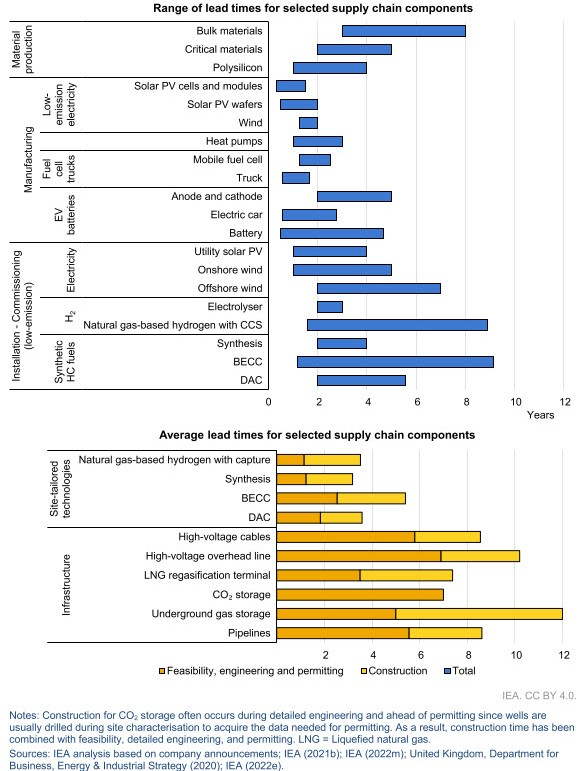
\includegraphics[width=0.8\textwidth]{Images/supply_chain/time_for_deploying_vis.jpg}
    \caption{Intervalle de temps de développement de capacité de production (haut), temps moyen de développement d'infrastructures (bas)}
    \label{fig:time_supplu}
\end{figure}
Le temps de développement de nouvelles unités de production pour les composants du photovoltaïque et de l'éolien peut aller jusqu'à 2 ans (figure \ref{fig:time_supplu}). Cependant, il est fréquent que plusieurs mois soient nécessaires pour atteindre la capacité nominale à cause de l'affinage du processus de fabrication. De manière similaire, une unité de production de batterie, d'anode ou de cathode se construit en moins de 5 ans et quelques mois sont nécessaires pour atteindre la capacité nominale.\smallbreak
L'assemblage de véhicules électriques peut souvent s'opérer dans une usine d'assemblage de véhicules thermiques rééquipée. Les procédés industriels pour l'assemblage sont matures et les capacités de productions sont souvent excédentaires.\smallbreak
La construction de nouvelles unités de raffinage de métaux critiques dure entre 2 et 5 ans. C'est moins long que la construction d'unités de production d'acier, d'aluminium ou de ciment dont la durée de construction s'étend de 3 à 8 ans.
